\chapter{Early Earth Chemistry with LAMMPS-ANI} 
\label{chapter4}

The integration of machine-learned interatomic potentials into large-scale molecular dynamics (MD) simulations is the primary objective of developing ANI-NNPs.
This does, however, introduce new challenges to ensure compatibility between force field-oriented dynamics software and TorchANI as a potential calculator.
Molecular dynamics simulation suites such as AMBER \cite{amber_overview} are famously scalable, offering multi-GPU support and efficient computation of neighbor lists, time step operations, and thermostat management.
However, this scalability is typically limited to running independent replicas of a system across multiple GPUs, rather than partitioning a single, extremely large system across multiple GPUs.
LAMMPS (Large-scale Atomic/Molecular Massively Parallel Simulator) \cite{lammps} is a natural choice for scaling dynamics simulations due to its efficient parallel computing capabilities. 
Unlike many other popular MD packages, LAMMPS is designed for domain decomposition \cite{lammps_original} and efficient distribution of workloads across multiple GPUs within a single node as well as across multiple compute nodes. 
This is essential for executing large-scale simulations, scaling into systems of millions of atoms. 
The modular and developer-friendly LAMMPS architecture seamlessly facilitates the incorporation of external potential models, making it an ideal platform for integrating TorchANI as a potential calculator.
The following chapter demonstrates the capability of massively scaled ANI-driven MD through the large-scale ``Early Earth" simulations of systems containing up to tens of millions of atoms.


\section{The Interface of TorchANI and LAMMPS}
\label{sec:lammps-ani}

To implement scalable and parallelized ANI-driven MD simulations, LAMMPS-ANI was developed by Dr. Jinze Xue \cite{lammps_ani} as a dynamic shared library plugin that seamlessly integrates ANI models into LAMMPS.\footnote{Parts of this chapter are adapted with permission from our upcoming manuscript: LAMMPS-ANI: Large Scale Molecular Dynamics Simulations with ANI Neural Network Potential \cite{lammps_ani}.}
The computational workflow is structured into three main components: the LAMMPS package, a LAMMPS-ANI C++ Interface, and the TorchANI neural network potential calculator. 
The MD setup and most of the computational tasks for dynamics is handled by LAMMPS, distributing across GPUs for efficient calculations of atomic motion, temperature regularization, and neighbor lists.
The LAMMPS-ANI C++ Interface initializes the ANI model on each GPU, ensuring that atomic position data is correctly formatted and transferred to the neural network for potential calculations.
This could be thought of as a rugged replacement for the force field (FF) used in driving dynamics.
In the current LAMMPS-ANI scheme, we neglect certain aspects that are important to force field-driven dynamics, notably partial charges and electrostatics.
While ANI models do not explicitly consider these aspects of potential energy calculation, the data used in training ANI models does consider these effects which allows the model to account for the contribution of atomic charges in a properly trained ANI model.

LAMMPS retrieves atom positions from neighboring domains at each time step and updates neighbor lists every ten steps, accounting for all necessary atomic interactions---including ghost atoms on the border between two domains.
A schematic example of domain decomposition and ghost atoms is given in Figure \ref{fig:ghost_atoms}.

\begin{figure}[!ht]
    \centering
    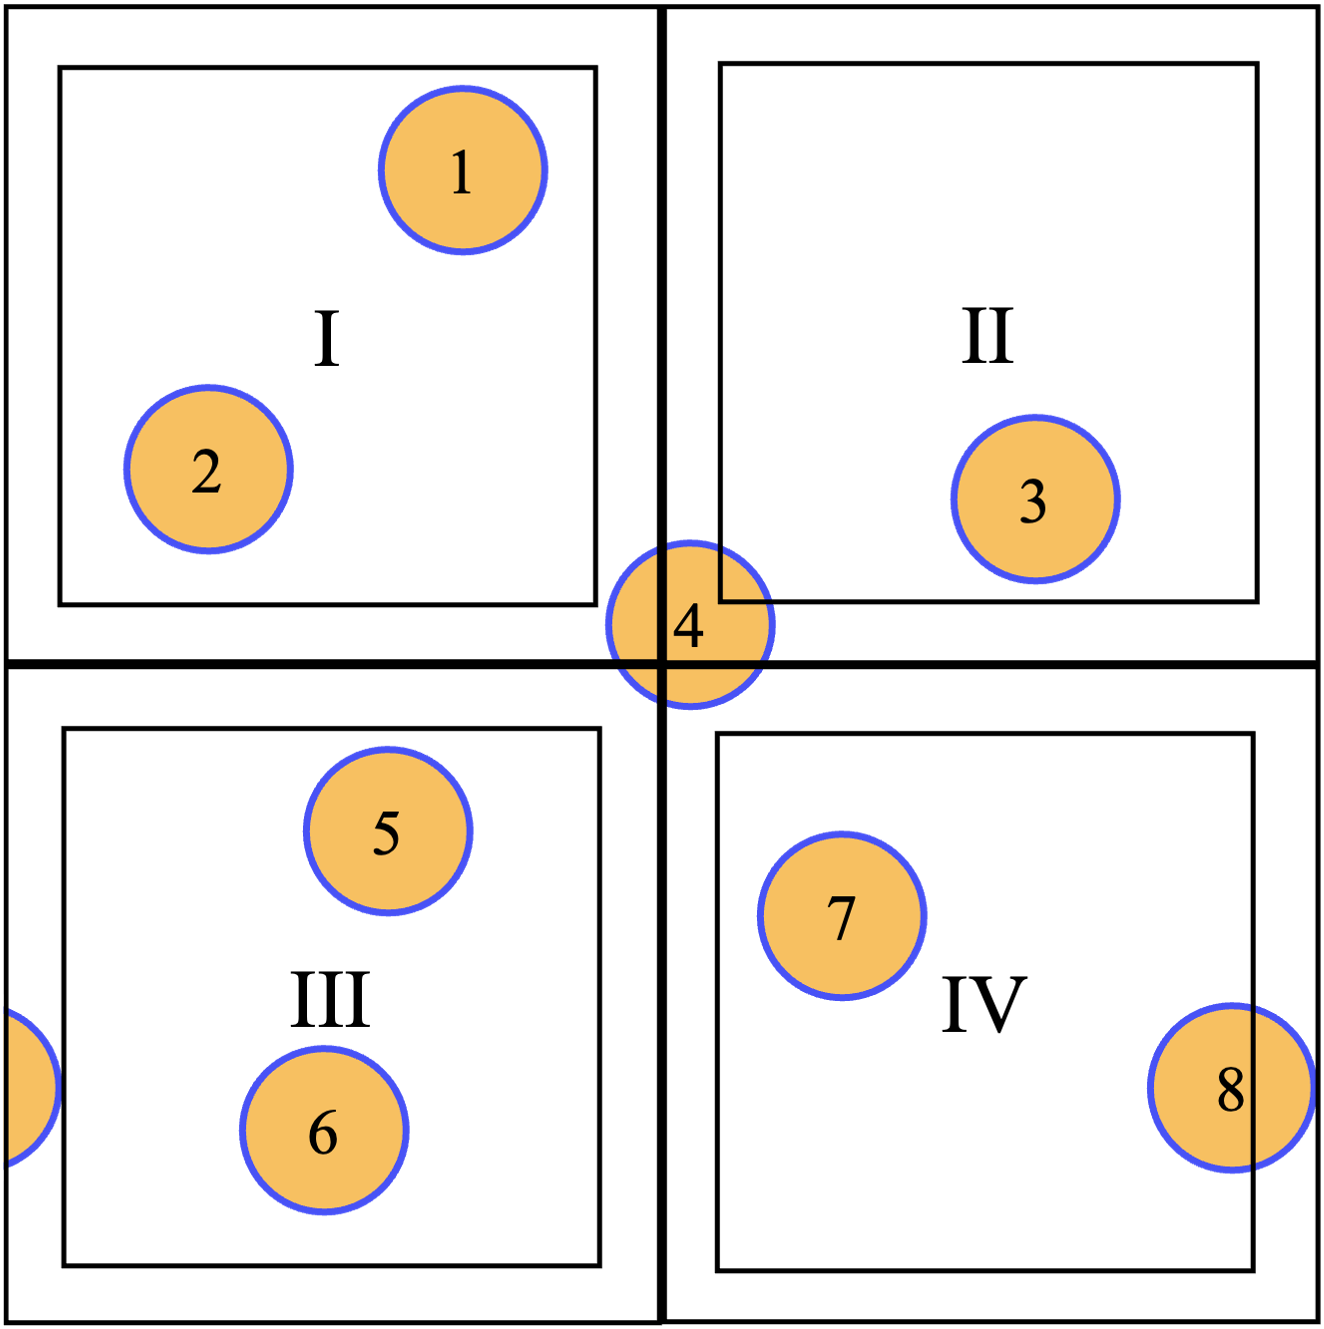
\includegraphics[width=.675\linewidth]{Images/ghost_atoms.png}
    \caption[Example of ghost atoms in domain decomposition]{Example of domain decomposition and ghost atoms. Note here that atoms 4 and 8 interact with atoms of neighboring domains.}
    \label{fig:ghost_atoms}
\end{figure}

The inclusion of ghost atoms within the AEV cutoff radius is critical to maintaining physically accurate predictions across domains.
Note in Figure \ref{fig:ghost_atoms} that atom indices [1, 2, 3, 5, 6, 7] are present only in their assigned domain, thus the interactions for these atoms are contained within a singular computational region.
However, atoms 4 and 8 are positioned along domain boundaries and must be accounted for in multiple domains to recreate the physicality of the interactions experienced by these atoms and the atoms in each of the respective regions.
Specifically, atom 8 is present in domains III and IV, and atom 4 must be replicated across all four domains.

Positional data, along with atomic identities, are processed by the ANI model, which constructs Atomic Environment Vectors (AEVs) to describe the local chemical environment. 
The ANI model then computes potential energies and derives atomic forces via automatic differentiation, distributing these force contributions back across atoms via the LAMMPS-ANI C++ Interface. 
The processed outputs—molecular energy, atomic forces, and stress tensors—are passed back into LAMMPS, which integrates the equations of motion to advance atomic positions. 
This cycle then repeats, allowing for long-timescale MD simulations powered by ANI for massively scaled systems.
By leveraging GPU parallelization and efficient data exchange, LAMMPS-ANI extends the applicability of machine-learned potentials to systems far larger than those used in training. 
Parallelization across GPUs relies on efficient implementation of CUDA-driven operations, notably CUDA-Accelerated Atomic Environment Vector (CUAEV) \cite{torchani_2.0} calculations.

A major bottleneck in ANI simulations is neighbor list generation, which originally relied on a brute-force method that scanned all atomic pairs within the cutoff. 
CUAEV introduces an optimized neighbor list algorithm that tracks only relevant atoms, drastically reducing memory usage for large systems. 
Additional optimizations, such as cell-list or Verlet-list algorithms \cite{allen_book}, further improve performance for large-scale simulations and, though that is outside of the scope of the work presented here, it is relevant for the massively-distributed simulation trajectory analysis discussed in Chapter \ref{chapter5}.
CUAEV replaces PyTorch’s tensor-based AEV computations with custom CUDA kernels optimized for memory-efficient parallel execution \cite{torchani_2.0}. 
Utilization of CUDA kernels enhance GPU performance by improving occupancy, minimizing atomic operations, and optimizing memory access patterns, resulting in significantly faster force evaluations. 
Forces in MD simulations are computed as the negative gradient of total energy with respect to atomic positions (Eqn. \ref{eq:force_dE}), requiring efficient automatic differentiation.
CUAEV optimizes this backward pass by streamlining derivative calculations while maintaining numerical accuracy. 
It also introduces an optimized double-backward computation for force training, reducing redundant calculations and improving scaling efficiency.

Many LAMMPS operations have traditionally been computed on CPU, even in GPU-accelerated simulations.
When using an interface for an external potential, such as TorchANI, this can require excessive communication between CPU-GPU.
Neighbor list computations, position updates, and thermostat updates are handled on CPU by default \cite{lammps, lammps_ani}.
As TorchANI uses GPUs to compute the potential at each time step, this requires repeatedly passing new positional data from CPU to the GPU, computing the potential, passing data back to the CPU for position updates and temperature equilibration. 
The recently developed KOKKOS \cite{kokkos} package in LAMMPS \cite{kokkos_exascale} is used to migrate operations that typically occur on CPU to the GPU, minimizing the required communication between these two processing units, which was a major bottleneck in early implementations of large-scale ANI dynamics simulations.

Benchmark tests on systems ranging from 100k to 100M atoms \cite{lammps_ani} demonstrate that LAMMPS-ANI scales efficiently with increasing GPU counts, particularly for large systems where communication overhead is minimized. 
Compared to other machine-learned potentials, such as Allegro \cite{allegro}, LAMMPS-ANI achieves significantly ($30-60\text{x}$) faster simulation speeds for massive-scale molecular dynamics \cite{lammps_ani}. 
With the help of GPU acceleration, optimized neural network inference, and efficient GPU-GPU communication, LAMMPS-ANI sets a new standard for scalable, machine-learned molecular simulations.
The utility of these advancements for scaling reactive prebiotic chemistry simulations up to tens of millions of atoms is explored in Section \ref{sec:miller_experiment} and the results of such a massive-scale simulation is the focus of Chapter \ref{chapter5}.

\section{ANI-1xnr}
\label{sec:ani-1xnr}

Conducting reactive molecular dynamics simulations presents significant challenges, requiring models that can accurately capture bond breaking and formation without relying on predefined reaction coordinates. 
Despite their computational efficiency, classical force fields are unable to model changes in chemical bonding, and quantum mechanical methods, though highly accurate, are computationally prohibitive for large-scale simulations. 

The ANI-1xnr model by Zhang, et al. \cite{ani-1xnr} was developed as an extension of the ANI family of neural network potentials to accurately model gas phase reactivity by incorporating transition-state and reactive molecular data into its training set.
ANI-1xnr builds upon the active learning framework established in ANI-1x, extended to a broader chemical space that includes transition-state geometries and high-energy molecular configurations. 
By incorporating such structures in the training set, ANI-1xnr shows the ability to generalize beyond near-equilibrium molecular structures, making it suitable for simulations where reactive events are expected to occur spontaneously.
This makes ANI-1xnr particularly well-suited for investigating complex reaction pathways in chemically rich environments, such as prebiotic chemistry, to model high-temperature reactions \cite{ani-1xnr}. 
Additionally, ANI-1xnr retains the scalability advantages of ANI models, enabling large-scale molecular dynamics simulations with thousands to millions of atoms while maintaining quantum mechanical chemical accuracy.

The efficient implementation of TorchANI as a potential calculator in LAMMPS facilitates GPU-accelerated reactive simulations, allowing for exploration of long-timescale chemical processes that would otherwise be inaccessible with traditional quantum chemistry methods.
In the next section, a specific application of ANI-1xnr is explored using LAMMPS-ANI: simulating the Miller-Urey experiment, a landmark study in prebiotic chemistry that demonstrated the abiotic synthesis of organic molecules under early Earth conditions. 

\section{The Miller-Urey Experiment}
\label{sec:miller_experiment}

The Miller-Urey experiment, conducted in 1952 \cite{miller_experiment}, was a landmark study demonstrating the abiotic synthesis of organic molecules under plausible early Earth conditions. 
By subjecting a gas phase mixture of methane ($\text{CH}_4$), ammonia ($\text{NH}_3$), hydrogen ($\text{H}_2$), and water ($\text{H}_2\text{O}$) to electrical discharges that simulated lightning, Miller and Urey observed the spontaneous formation of amino acids, nucleobase precursors, and other complex organic compounds \cite{miller_experiment}. 
This provided crucial evidence that the building blocks for biomolecules could emerge from simple molecular precursors given the right environmental conditions.

Simulating the full chemical complexity of such a system using chemically accurate QM approaches is computationally infeasible due to the number of molecules (and, therefore, electrons) and the timescale required to uncover the complex reaction pathways involved.
ANI-1xnr stands out as an efficient alternative, enabling large-scale simulations that capture bond-breaking and bond-forming events with near-QM accuracy. 
This was first demonstrated by Zhang et al. \cite{ani-1xnr} with a small-scale ANI-1xnr simulation of a 228-atom system, replicating key aspects of the Miller-Urey experiment. 
This benchmark study confirmed the model’s ability to drive reaction dynamics and demonstrate the formation of organic molecules without explicitly considering electronic behavior.


\subsection{CUDA-Accelerated Molecule Finder}
\label{subsec:molfind}

Before a discussion of the results of increasingly scaled-up reactive molecular dynamics simulations, we must introduce the tool used to detect changes in bonding throughout each run.
The CUDA-accelerated Molecule Finder, or \verb|molfind|, is a protocol written in Python with \verb|RAPIDS| \cite{rapids} for GPU-accelerated data analysis of trajectory data.
This program operates by translating each simulation snapshot into a graph data structure on the GPU, where atoms are represented as graph nodes and pairwise interactions (\textit{e.g.}, bonds, detected via distances between atoms) are edges. 
Table \ref{tbl:bond_distances} shows the bond distances used to determine connectivity.
An additional stretch buffer of 0.2 \angstrom is added to each of the distances in Table \ref{tbl:bond_distances} to account for distorted geometries at very high temperatures.
This stretch buffer runs a small risk of including nearby atoms that are not bonded, but even in very large simulations (as explored in Chapter \ref{chapter5}), we see that this is a negligible amount of fragments detected.

\begin{table}[h!]
\centering
\caption[Interatomic distances used in determining connectivity]{Interatomic distances used in determining connectivity.
}\label{tbl:bond_distances}
\begin{tabularx}{0.265\textwidth}{l r}  
\toprule
Species & Distance $(\angstrom)$ \\
\midrule
H-H & 0.75 \\
H-C & 1.09 \\
H-N & 1.01 \\
H-O & 0.96 \\
C-C & 1.54 \\
C-N & 1.43 \\
C-O & 1.43 \\
N-N & 1.45 \\
N-O & 1.47 \\
O-O & 1.48 \\
\bottomrule
\end{tabularx}
\end{table}

To construct graphs of connected components, the tool uses GPU-based neighbor-list building using cell-lists and the cuGraph library to create and store the adjacency information in GPU memory. 
The next step in \verb|molfind| is to get the chemical formula of each connected component to identify sets of atoms that form discrete molecular fragment by collecting and sorting atomic species, which helps identify the basic stoichiometry.
The fragment graphs are then filtered to only connected components with formulas matching a prebuilt reference database of molecular graphs of interesting molecules (amino acids, dipeptides, sugars, and other small biomolecules).
The initial list of molecules of interest is given in Table \ref{tbl:molfind_targets}. 
This table excludes dipeptides, which encompass all possible pairs of the amino acids listed.
We refer to this list of molecules as the PubChem dataset, as the 2D structures for each of the named molecules on this list were obtained via PubChem \cite{pubchem}.

\begin{table}[h!]
\centering
\caption[Initial list of interesting molecules]{Initial list of interesting molecules including nitrogenous bases, sugars, fatty acids, and 18 of the 20 essential proteogenic amino acids.
}\label{tbl:molfind_targets}
\begin{tabularx}{0.49\textwidth}{l l l}  
\toprule
Molecule & Formula & Category \\
\midrule
Adenine  &   C\textsubscript{5}H\textsubscript{5}N\textsubscript{5} & Nucleobases \\
Guanine  &  C\textsubscript{5}H\textsubscript{5}N\textsubscript{5}O & Nucleobases \\
Cytosine  &  C\textsubscript{4}H\textsubscript{5}N\textsubscript{3}O & Nucleobases \\
Thymine  & C\textsubscript{5}H\textsubscript{6}N\textsubscript{2}O\textsubscript{2} & Nucleobases \\
Uracil  & C\textsubscript{4}H\textsubscript{4}N\textsubscript{2}O\textsubscript{2} & Nucleobases \\
Glucose  &  C\textsubscript{6}H\textsubscript{12}O\textsubscript{6} & Sugars \\
Fructose  &  C\textsubscript{6}H\textsubscript{12}O\textsubscript{6} & Sugars \\
Ribose  &  C\textsubscript{5}H\textsubscript{10}O\textsubscript{5} & Sugars \\
Deoxyribose  &  C\textsubscript{5}H\textsubscript{10}O\textsubscript{4} & Sugars \\
Caprylic acid  &  C\textsubscript{8}H\textsubscript{16}O\textsubscript{2} & Fatty acids \\
Capric acid  & C\textsubscript{10}H\textsubscript{20}O\textsubscript{2} & Fatty acids \\
Lauric acid  & C\textsubscript{12}H\textsubscript{24}O\textsubscript{2} & Fatty acids \\
Myristic acid  & C\textsubscript{14}H\textsubscript{28}O\textsubscript{2} & Fatty acids \\
Palmitic acid  & C\textsubscript{16}H\textsubscript{32}O\textsubscript{2} & Fatty acids \\
Alanine  &    C\textsubscript{3}H\textsubscript{7}NO\textsubscript{2} & Amino acids \\
Arginine  &  C\textsubscript{6}H\textsubscript{14}N\textsubscript{4}O\textsubscript{2} & Amino acids \\
Asparagine  &   C\textsubscript{4}H\textsubscript{8}N\textsubscript{2}O\textsubscript{3} & Amino acids \\
Aspartic Acid  &    C\textsubscript{4}H\textsubscript{7}NO\textsubscript{4} & Amino acids \\
Glutamine  &  C\textsubscript{5}H\textsubscript{10}N\textsubscript{2}O\textsubscript{3} & Amino acids \\
Glutamic Acid  &    C\textsubscript{5}H\textsubscript{9}NO\textsubscript{4} & Amino acids \\
Glycine  &    C\textsubscript{2}H\textsubscript{5}NO\textsubscript{2} & Amino acids \\
Histidine  &   C\textsubscript{6}H\textsubscript{9}N\textsubscript{3}O\textsubscript{2} & Amino acids \\
Isoleucine  &   C\textsubscript{6}H\textsubscript{13}NO\textsubscript{2} & Amino acids \\
Leucine  &   C\textsubscript{6}H\textsubscript{13}NO\textsubscript{2} & Amino acids \\
Lysine  &  C\textsubscript{6}H\textsubscript{14}N\textsubscript{2}O\textsubscript{2} & Amino acids \\
Phenylalanine  &   C\textsubscript{9}H\textsubscript{11}NO\textsubscript{2} & Amino acids \\
Proline  &    C\textsubscript{5}H\textsubscript{9}NO\textsubscript{2} & Amino acids \\
Serine  &    C\textsubscript{3}H\textsubscript{7}NO\textsubscript{3} & Amino acids \\
Threonine  &    C\textsubscript{4}H\textsubscript{9}NO\textsubscript{3} & Amino acids \\
Tryptophan  & C\textsubscript{11}H\textsubscript{12}N\textsubscript{2}O\textsubscript{2} & Amino acids \\
Tyrosine  &   C\textsubscript{9}H\textsubscript{11}NO\textsubscript{3} & Amino acids \\
Valine  &   C\textsubscript{5}H\textsubscript{11}NO\textsubscript{2} & Amino acids \\
\bottomrule
\end{tabularx}
\end{table}

The fragment graphs are then sorted by chemical formula and the formulas which match entries of the PubChem dataset are compared with a CPU-based graph isomorphism check using the \verb|NetworkX| \cite{networkx} library to verify exact structural matches against a reference structure.
Finally, two output data frames are produced, referred to as \verb|df_formula| and \verb|df_molecule|.
The first of these, \verb|df_formula|, contains every chemical formula that appears in a frame when it is fragmented into subgraphs, and counts how many times each formula appeared.
The other, \verb|df_molecule|, stores the names and atom indices of fragments which match a reference graph.

This approach is far more efficient than trying to name each molecule independently (\textit{i.e.}, via RDKit \cite{rdkit}), which would have a cost on the order of seconds per molecule.
For long trajectories, or frames with millions of atoms, a per-molecule naming approach would make this analysis computationally prohibitive.
By keeping the operations of graph-building, connected component search, and string preprocessing to filter out uninteresting data on the GPU, \verb|molfind| can scale to tens of millions of atoms, enabling us to quickly sweep through trajectory data in order to track how molecular species evolve over time and detect rare or unexpected products in large reactive systems.

\subsection{The Small Early Earth System}
\label{subsec:small_system}

Replicating the simulation conducted by Zhang, et al., we start with a system setup of 70 molecules, listed in Table \ref{tbl:228_sim_counts}.
This mixture is similar to that of the Miller-Urey experiment, with the addition of carbon monoxide as an additional source of carbon and oxygen atoms.
Despite being a very large system for \textit{ab initio} molecular dynamics, we refer to this as the ``small'' system as we scale toward simulations of millions of atoms.

\begin{table}[h!]
\centering
\caption[Starting molecules in 228 atom Early Earth simulation]{Starting molecules in the small atom Early Earth simulation.
}\label{tbl:228_sim_counts}
\begin{tabularx}{0.315\textwidth}{lrr}  
\toprule
Species & $N_\text{molecules}$ & $N_\text{atoms}$ \\
\midrule
$\text{H}_2$ & 16 & 32 \\
$\text{H}_2\text{O}$ & 14 & 42 \\
CO & 14 & 28 \\
$\text{NH}_3$ & 14 & 56 \\ 
$\text{CH}_4$ & 14 & 70 \\
Total & 70 & 228 \\
\bottomrule
\end{tabularx}
\end{table}

The starting topology for the system was generated from optimized geometries of the starting materials
($\text{H}_2$, $\text{H}_2\text{O}$, CO, $\text{NH}_3$, $\text{CH}_4$)
with \verb|PACKMOL| \cite{packmol} to efficiently distribute the 70 molecules throughout at cubic simulation box with 12.1 $\angstrom$ edges.
Molecular dynamics for this small, 228 atom system was conducted with LAMMPS-ANI over 4.4 ns, using a 0.25 fs timestep and saving positions every 50 frames, to investigate the effects of extreme temperatures on reaction dynamics.
The system is first heated from 0 K to 300 K over 100 ps, then rapidly ramped to 2500 K over the next 100 ps, where it remains for 4 nanoseconds, allowing bond rearrangements and potential chemical reactions to occur. 
Finally, the system is cooled back to 300 K over 100 ps and allowed to relax at 300 K for the last 100 ps, mimicking quenching conditions.
This setup enables the study of reaction pathways and thermal stability under high-temperature conditions relevant to prebiotic chemistry and extreme planetary environments.
The starting geometry and final frame positions are visualized using VMD \cite{vmd} in Figure \ref{fig:228_atom_run}.  

\begin{flushleft}
\begin{multiFigure}
    \addFigure{0.495}{Images/early_earth/cropped_228_initial.png}
    \addFigure{0.495}{Images/early_earth/cropped_228_final.png} \\
\captionof{figure}[228 atom early earth system]{228 atom Early Earth system (A) before and (B) after running dynamics for 4.4 ns; note in the final geometry that some hydrogen atoms appear far from the molecules to which they're bound due to periodic boundary conditions.
}
\label{fig:228_atom_run}
\end{multiFigure}
\end{flushleft}

Table \ref{tbl:228_final_sim_counts} shows the species detected by \verb|molfind| at the final frame of the simulation.
Here, we can see that the total number of molecules has decreased---even with a handful of free hydrogen atoms floating about. 


\begin{table}[h!]
\centering
\caption[Molecules in the final frame of the 228 atom run]{Molecules found in the final frame of the small atom Early Earth simulation.
}\label{tbl:228_final_sim_counts}
\begin{tabularx}{0.32\textwidth}{lrr}  
\toprule
Formula & $N_\text{molecules}$ & $N_\text{atoms}$ \\
\midrule
NH\textsubscript{4} & 7 & 35 \\
C\textsubscript{3}H\textsubscript{8} & 1 & 9 \\
C\textsubscript{3}H\textsubscript{10} & 2 & 22 \\
H & 5 & 5 \\
CNO & 1 & 3 \\
CHNO & 1 & 4 \\
NH\textsubscript{3} & 5 & 20 \\
CO\textsubscript{2} & 3 & 9 \\
CO & 4 & 8 \\
HO & 1 & 2 \\
CH\textsubscript{4} & 10 & 50  \\
H\textsubscript{2}O & 15 & 45 \\
H\textsubscript{2} & 8 & 16 \\
Total & 63 & 228 \\
\bottomrule
\end{tabularx}
\end{table}

This trend can also be seen by plotting the total energy of the simulation versus temperature, as shown in Figure \ref{fig:228_atom_energy_plots}.
There are two distinct regions of potential energy (and, thus, total energy) as the system is heating and cooling---corresponding to the upper and lower curves respectively.\\
\bigskip

\begin{multiFigure}
    \begin{minipage}{\linewidth}
        \centering
        \addFigure{0.9}{Images/228_tot_eng.png}
    \end{minipage}
    \addFigure{0.5}{Images/228_pot_eng.png}
    \addFigure{0.5}{Images/228_kin_e.png}
\captionof{figure}[228 atom simulation: energy versus temperature]{
(A) Total energy (kcal/mol) versus temperature (K);
(B) Potential energy (kcal/mol) and (C) kinetic energy (kcal/mol) versus  versus temperature (K) across the 4.5 nanosecond simulation of a 228 atom Early Earth system.
}
\label{fig:228_atom_energy_plots}
\end{multiFigure}

Due to having fewer molecules and, therefore, more chemical bonds, the total energy across the simulated system is lower after dynamics are ran for 4.4 nanoseconds.
The exact run shown in Figure \ref{fig:228_atom_energy_plots} did not produce any novel molecules of interest, though other MD runs with the same system setup showed two appearances of glycine throughout the simulation \cite{lammps_ani}.
The major limitation of exploring possible reaction pathways with molecular dynamics is sampling: either the size of the system or the time scale must be extended in order to efficiently sample chemical space.
The next step in scaling this system up was to increase the size by a factor of a thousand, in what we refer to as the ``medium'' system.


\subsection{The Medium Early Earth System}
\label{subsec:medium_system}

Using the same approach described in Subsection \ref{subsec:small_system}, the Early Earth system was scaled up by a factor of $10^3$ to a cubic box with edge lengths of 121 \angstrom.
This system was prepared, like the 228 atom system, with \verb|PACKMOL| to distribute the starting materials throughout the box.
The species present at the start of this trajectory are provided in Table \ref{tbl:228k_start_counts}.

\begin{table}[h!]
\centering
\caption[Molecules in the first frame of the 228,000 atom run]{Molecules present in the start frame of the medium atom Early Earth simulation.
}\label{tbl:228k_start_counts}
\begin{tabularx}{0.33333\textwidth}{lrr}  
\toprule
Species & $N_\text{molecules}$ & $N_\text{atoms}$ \\
\midrule
$\text{H}_2$ & 16,000 & 32,000 \\
$\text{H}_2\text{O}$ & 14,000 & 42,000 \\
CO & 14,000 & 28,000 \\
$\text{NH}_3$ & 14,000 & 56,000 \\ 
$\text{CH}_4$ & 14,000 & 70,000 \\
Total & 70,000 & 228,000 \\
\bottomrule
\end{tabularx}
\end{table}

The molecular dynamics simulation of this medium-sized Early Earth system was conducted, following the same protocol as described in Subsection \ref{subsec:small_system} with a 0.25 fs timestep and saving every 50 frames, by heating the initial geometry from 0-300 K over 100 ps, rapidly heating from 300-2500 K over the next 100 ps, then the temperature is held at 2500 K for 4.0 ns.
The run detailed here ended early, before the final cooling due to a time constraint.
The bulk of the trajectory data (4.04 ns) was saved, thus we moved on to scaling the system further, as this trajectory was sufficient to conduct \verb|molfind| benchmark studies.

Unlike the small system, which can easily be visually inspected frame-by-frame, at this scale we can not hope to get useful information out of this by inspecting in VMD \cite{vmd}, leading us to develop and refine GPU-accelerated data analysis protocols.
The starting and final frame geometries are provided in Figure \ref{fig:228000_atom_run}, where the system largely appears as a featureless mass of atoms. 

\begin{flushleft}
\begin{multiFigure}
    \addFigure{0.5}{Images/early_earth/228000-start.png}
    \addFigure{0.5}{Images/early_earth/228000-after.png} \\
\captionof{figure}[228,000 atom early earth system]{
(A) Before and (B) after running dynamics on a 228,000 atom Miller experiment system for 2 ns.
}
\label{fig:228000_atom_run}
\end{multiFigure}
\end{flushleft}

The analysis of this system was conducted with a rudimentary version of \verb|molfind|, before the refinements described throughout Chapter \ref{chapter5} were implemented.
As such, we report on the molecules with formulas that match those of reference molecules, but this should not be taken as an assumption that the molecules identified in this way are absolute matches for the molecules of interest listed in Table \ref{tbl:molfind_targets}.
Throughout this 4.04 ns simulation, 7,756 unique chemical formulas appeared at least once.
A truncated account of the unique chemical formulas present in the final frame of the simulation are given in Table \ref{tbl:228k_final_counts}, where most of the data has been omitted due to the sheer number of unique fragments present.


\begin{table}[h!]
\centering
\caption[Chemical formulas in the final frame of the 228,000 atom run]{Molecular formulas found in the final frame of the medium atom Early Earth simulation.
}\label{tbl:228k_final_counts}
\begin{tabularx}{0.455\textwidth}{lrr}  
\toprule
Formula & $N_\text{molecules}$ & $N_\text{atoms}$ \\
\midrule
C\textsubscript{5}H\textsubscript{10}O\textsubscript{2} & 2 & 26 \\
C\textsubscript{1}H\textsubscript{4}N\textsubscript{2}O & 9 & 63 \\
C\textsubscript{8}H\textsubscript{18}O & 1 & 18 \\
C\textsubscript{5}H\textsubscript{11}NO\textsubscript{2} & 1 & 16 \\
C\textsubscript{6}H\textsubscript{13}NO & 1 & 18 \\
... & ... & ... \\
CH\textsubscript{2}N & 58 & 232 \\
C\textsubscript{2}HNO\textsubscript{3} & 2 & 14 \\
C\textsubscript{2}H\textsubscript{4} & 80 & 400 \\
C\textsubscript{7}H\textsubscript{14}O & 3 & 45 \\
C\textsubscript{4}H\textsubscript{9}NO & 2 & 22 \\
Total: 518 formulas & 67,207 & 228,000 \\
\bottomrule
\end{tabularx}
\end{table}

The total appearances of formulas matching our list of named molecules is provided in the Appendix Table \ref{tbl:228k_mol_counts}, along with the maximum times that formula appeared in a single frame.
The chemical formula for glycine is the most commonly detected, showing up 118,675 times, while formulas matching adenine and ribose appear only once throughout the entire run.
Bear in mind that many appearances of formulas that match molecules in our PubChem dataset are double-counted due to the molecule persisting for many timesteps after formation.

This run, like the small system, primarily served as a proof of concept and as benchmark systems, thus the results of \verb|molfind| exact structure matching and the total counts are omitted.
This run showed, in line with our expectations, that the synthesis of small organic molecules and biological precursors is far more common as the system is scaled up.
Expanding the system to a larger simulation box with more interacting species effectively replaces the need for extended timescales to model the prebiotic chemistry in an Early Earth atmospheric environment.
With these promising results, we scaled the system up to an overall system size of 22.8 million atoms.



\subsection{The Early Earth Hero Run}
\label{subsec:hero_run_simulation}

The system preparation for a massive system is far more computationally intensive than the process described previously, though the methods remain the same.
The system described here was prepared and initial simulations were conducted by Dr. Jinze Xue in December of 2023 on an exclusive reservation of all 1,048 GPUs on the HiPerGator (HPG) supercomputer.
Using \verb|PACKMOL|, distributing the five starting components ($\text{H}_2$, $\text{H}_2\text{O}$, CO, $\text{NH}_3$, $\text{CH}_4$) throughout the cubic simulation box $(l=512 \ \angstrom)$ took 69,416 seconds, or a bit over 19 hours to generate a starting topology.
This was only the beginning of the complications encountered with the resource-intensive nature of running and analyzing simulations at this scale. 
Timings for the small, medium, and Hero Run simulations are provided in Table \ref{tbl:md_timings}.

\begin{table}[h!]
\centering
\caption[Simulation timings for small, medium, and hero run simulations]{Simulation timings for small, medium, and hero run Early Earth simulations, including the total number of steps in each run, the total wall time, timesteps per second, and nanoseconds per day.
}\label{tbl:md_timings}
\begin{tabularx}{0.625\textwidth}{lrrr}  
\toprule
Timing & 228 atoms & 228k atoms & 22.8M atoms \\
 & (1 GPU) & (8 GPUs) & (1048 GPUs) \\
\midrule
Total steps & 17,600,000 & 16,165,000 & 17,600,000 \\
Total wall time & 18:34:41 & 55:50:15 & 168:42:37 \\
Steps/sec & 266.80 & 80.421 & 28.98 \\
ns/day & 5.763 & 1.737 & 0.626 \\
\bottomrule
\end{tabularx}
\end{table}

Note that the difference in total steps for the medium-sized system is due to the simulation ending earlier than expected as mentioned in Subsection \ref{subsec:medium_system}; initial timing benchmarks showed a slightly higher rate of steps per second than seen here, which led to an insufficiently short time requested in the SLURM job used to run dynamics.
However, this run was sufficiently long to compare timing with the small and large systems.
Another test, using only 4 A100 GPUs for the medium-sized system showed a rate of approximately 0.49 ns/day, suggesting that distributing the system more leads to large speedups simulation time. 

The Hero Run trajectory from this initial simulation occupies approximately 92 terabytes of disk space on a special allocation of \verb|red| storage on HPG. 
The simulation followed the same stages outlined in Subsection \ref{subsec:small_system}, heating from 0-300 K over 100 ps, 300-2500 K over the next 100 ps, running for 4 ns at 2500 K, and a final cooling to 300 K over the last 200 ps.
The trajectory was saved every 0.1 ns as the simulation was conducted, with each of the 44 trajectory files occupying a bit over 2 TB.
The size of these trajectory files means that an iterative approach to data processing must be implemented in order to extract any useful data. 
As with the medium system, inspecting this system visually is a wasted effort.
Unlike the medium-sized system, attempting to even load a single frame of the Hero Run trajectory causes VMD to crash.
Without extracting specific coordinates of interest from the simulation trajectory, we are unable to visualize any of this data.

This reactive simulation stands to reveal rare and complex reaction pathways that would be impossible to observe in smaller-scale studies. 
However, the sheer amount of data produced by this simulation introduced a new challenge: efficiently analyzing over a hundred terabytes of molecular trajectory data. 
The following chapter details the GPU-accelerated data analysis pipelines developed to extract meaningful chemical insights from this data, and explores how we can use large-scale simulations for sampling new data to fill the gaps in understanding of ML models in chemistry. 
